\documentclass[a4paper,twocolumn]{article}

\usepackage[utf8]{inputenc}
\usepackage[english]{babel}
\usepackage{graphicx}
\usepackage{caption}
\usepackage[left=2cm, right=2cm, top=2cm, bottom=2cm]{geometry}
\usepackage{amsmath}

\title{Panorama reconstruction using homographies}

\author{
	Sébastien Klasa - Polytech Paris-Sud\\
	\texttt{klasa.sebastien@gmail.com}
}

\date{28 October 2018}

\begin{document}
	
\maketitle

\begin{abstract}
	As part of the image processing course in the fifth year of engineering school Polytech Paris-Sud, this project aims to reconstruct a panorama from several photographs by finding homographies between pairs of images. As the purpose of the project is to understand the construction of panoramas, we implemented all algorithms ourselves. However, we use the OpenCV library to open, save and display images. We divided the project into four parts: detecting corners using the FAST detector, pairing them, finding the homography and finally constructing the panorama by transforming the images.
\end{abstract}

\section{FAST detector}

The first step of constructing a panorama is to find corners (i.e. interest points) in two overlapping images in a way that some of the corners corresponds to the same regions in both images. There are many methods of corner detection and we chose FAST (Features from Accelerated Segment Test) for its easy implementation. I implemented the naive version of the algorithm: for each pixel $p$ a circle of radius 3 is considered, if in this circle exists at least $n$ contiguous pixels which intensities are all higher or all lower than the intensity of $p$, it is labeled as a corner. I use a threshold $t$ such as for a pixel $x_i$ in the circle, if $I(p) - t \le I(x_i) \le I(p) + t$ then $x_i$ and $p$ have the same intensity. By formalizing, a pixel $p$ is a corner if one of this two conditions is met:

\begin{align*}
\exists S | \forall x \in S, I(x) \le I(p) - t\\
\exists S | \forall x \in S, I(x) \ge I(p) + t
\end{align*}

where $S$ is a set of $n$ contiguous pixels in the circle.
\\

I tested my implementation by comparing the result to the FAST detector implemented in OpenCV. Figures \ref{my_fast} and \ref{opencv_fast} are the comparison of the result of my FAST implementation and the OpenCV one using the parameters $n = 12$ and $t = 50$. We can see in those two images that the same corners are detected but my implementation detects less of them: this is probably due to a different method of non-maxima suppression. Another interesting comparison can be the execution time: for this image, OpenCV found corners in less than 5 ms and my implementation took about 500 ms. The execution time my algorithm is slower because I implemented the naive version, which could be improved by examining 4 example pixels and rejecting non-corners before searching the contiguous pixels.

\begin{figure}[h]
	\centering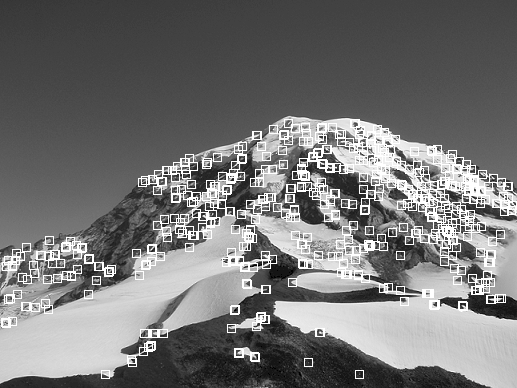
\includegraphics[width=0.5\textwidth]{images/fast/my_fast.png}
	\caption{Result of my implementation of the FAST detector.}
	\label{my_fast}
\end{figure}

\begin{figure}[h]
	\centering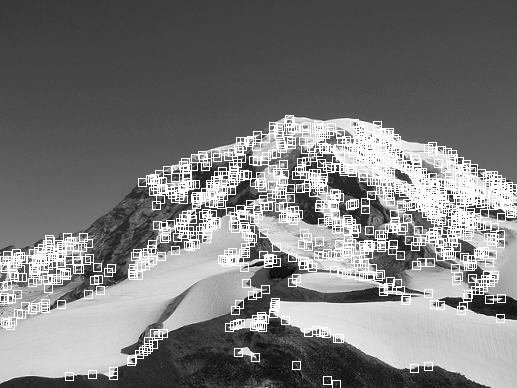
\includegraphics[width=0.5\textwidth]{images/fast/opencv_fast.png}
	\caption{Result of the OpenCV FAST detector.}
	\label{opencv_fast}
\end{figure}

\end{document}